\begin{document}
%intro

A recent article by SVT Nyheter showed which season is was on the $1^\text{st}$ of November for different areas in Sweden, as can be seen in Fig. \ref{fig:SVT}. According to this article it was already winter in the north of Sweden while in the most south part, including Lund, it was still summer. This did not seem to correspond to what one might observe when looking out the window in Lund, the ground was already covered with red leaves even though it was still summer according to SVT Nyheter. So which definitions of the season are there? Using one of these definitions when do the seasons start in Lund and how does the start of each season vary over a number of years?

\begin{figure}[h!]
\centering
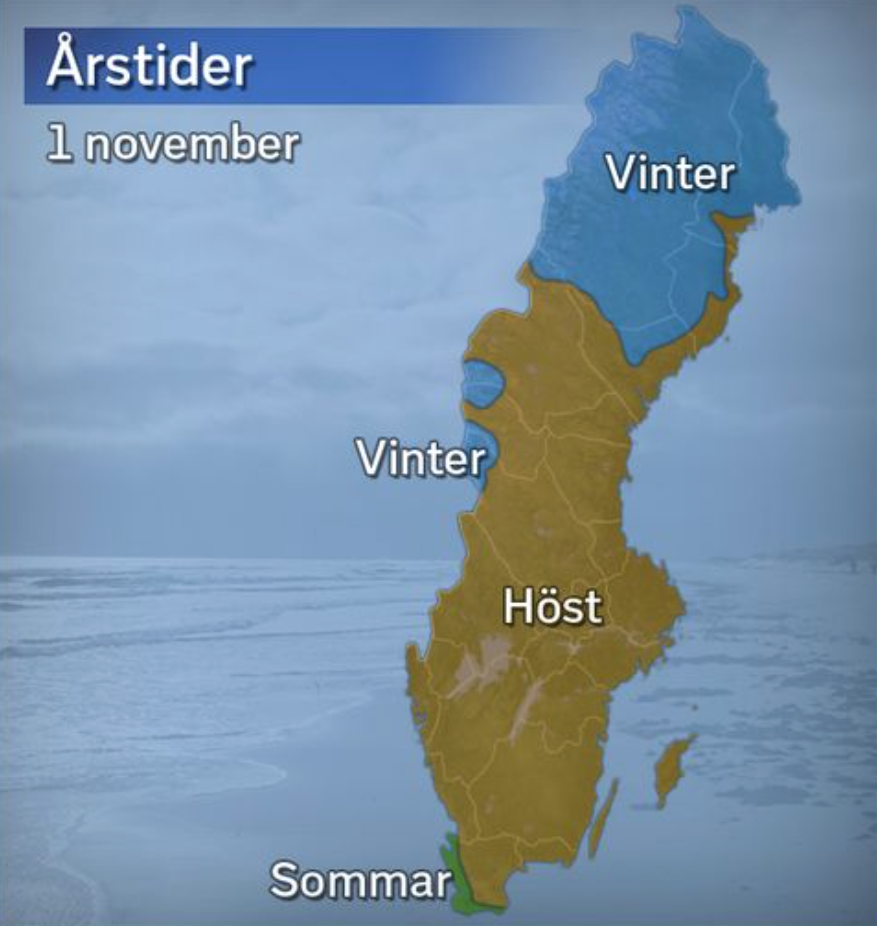
\includegraphics[width=0.4\textwidth]{SVT_seasons.png}
\caption{The season in different areas in Sweden on the $1^\text{st}$ of November. Image from \cite{SVT}.}
\label{fig:SVT}
\end{figure}

\subsection{Definition of the Seasons}
%\cite{SMHI}

Sveriges meteorologiska och hydrologiska institut (SMHI) uses two different definitions of the seasons, a definition based on the calendar and a meteorological definition \cite{SMHI}. According to the definition based on the calendar spring is always from March to May, summer from June to August, fall from September to November and winter from December to February. This is clearly the same for each year and is not dependent on temperature of any other parameter. The meteorological definition of the seasons is based on the average temperature of each day and the seasons can therefore be start on different dates each year. The meteorological winter starts when the average temperature of a day is equal to or below zero for 5 days in a row. The first day of winter is then the first of these 5 days.  The definition for the meteorological summer is similar, but the average temperature needs to be 10 degrees or higher. The meteorological spring starts when the average temperature of a day is between zero and 10 degrees for 7 days in a row. The definition for the meteorological fall is similar, but the temperature only need to be between zero and 10 degrees for 5 days in a row. The seasons do of course need to occur in the right order, which means that spring has to start after winter and fall has to start after summer. SMHI's meteorological definition of the seasons will be used for the data analyses. 

\subsection{Method}

\begin{wrapfigure}{R}{0.35\textwidth}
%\caption{something}
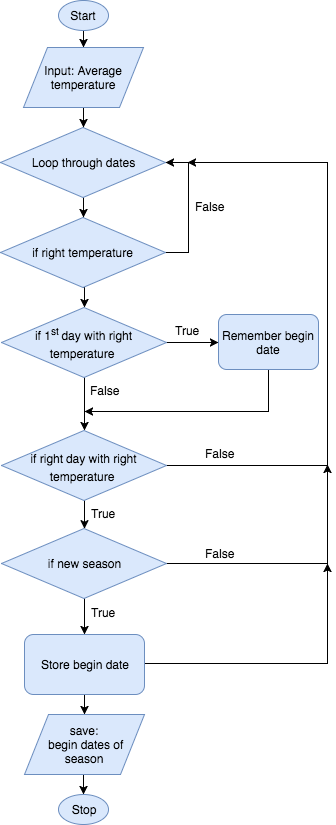
\includegraphics[scale=0.45]{start_season_diagram.png}
\caption{The code used for the calculation of the start of a season represented in a flowchart.}
%\caption{The code used for the calculation of the start of a season represented in a flowchart.}
\label{fig:flowchart}
\end{wrapfigure}

The temperature data of Lund from Sveriges meteorologiska och hydrologiska institut (SMHI) will be used to determined to beginning of the meteorological season for the years in the dataset.  The code used to produce the results on the beginning of the seasons can be found in \texttt{tempSeasons.cpp}, a number of member functions defined in \texttt{tempTrender.cpp} are also used.  The main function, which calls all other functions, of the section is \texttt{tempTrender::startDaySeasons}.  The first thing this function does is reading the data on Lund into a 2D vector with the use of \texttt{tempTrender::readData}. Since the meteorological definition of the seasons depends on the average temperature of a day, this is then calculated for every day in the dataset by  \texttt{calcAverageTemp}. Using the resulting average temperatures each first day of a season is determined for all seasons and years in the dataset. This is done using the function \texttt{tempTrender::beginningWinter} for winter,  \texttt{tempTrender::beginningSummer} for summer and \texttt{tempTrender::beginningSpringFall} for both spring and fall. \todo{merge functions} These functions are member variables since they use a member funtion \texttt{tempTrender::getDayOfYear}. The general flowchart of how each first day of all seasons is determined can be seen in \ref{fig:flowchart}. With the right temperature the temperature condition for a certain season is meant, which is smaller or equal to 0 degrees for winter, greater or equal to 10 degrees for summer and between 0 and 10 degrees for spring and fall. With the right day the condition on the number of subsequent is meant, which is 7 days for spring and 5 days for all other seasons. When a new season starts differs a lot between the seasons, for summer the only condition is that it occurs in a different year than the previous summer, because there is one summer per year. For spring and fall there is another condition that also needs to be satisfied, namely spring needs to occur after the first day of winter and fall needs to occur after the first day of summer. Because winter can cover part of the end of one year as well as the beginning of the next, winter does not always start once per year. There are four ways the first day of two consecutive winters can succeed each other. 
\newline

\begin{enumerate}
\item The successive winters are both early in the year (before June)
\item The successive winters are both late in the year (after June)
\item The successive winters are in the same year (one early in the year the other late)
\item The successive winters skip a year (one winter late in the year, the next early)
\end{enumerate}

If one of these cases is satisfied it is a new winter. Using the result for each season a bar graph showing the first day of the season as a function of the year is created by \texttt{plotSeason}. Histograms of the results are also created for each season using \texttt{histogram}. 

\subsection{Results}
%The date is represented by the day of the year (i.e. from 1 to 365 or 366).

\begin{figure}[ht!]
\centering
\subfloat[Bar graph]{\label{fig:spring_bar}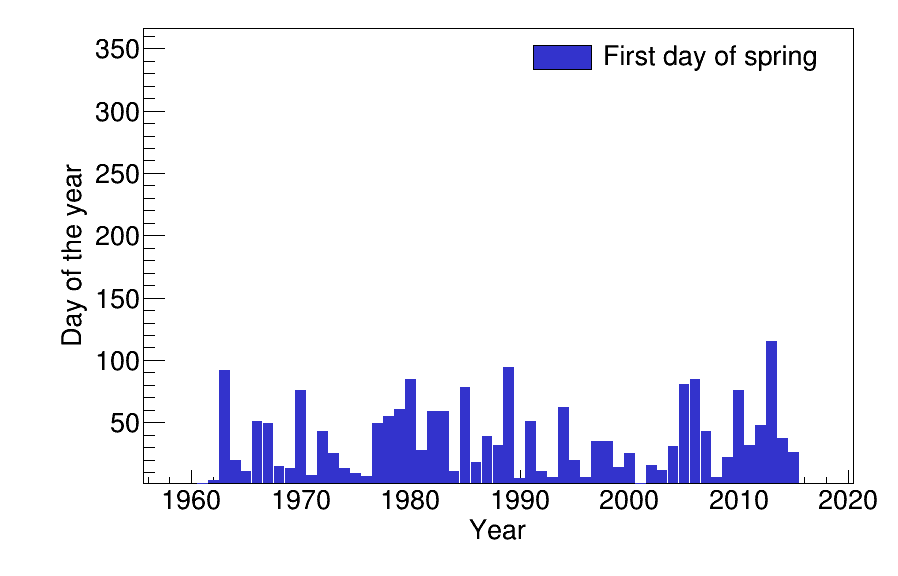
\includegraphics[width=0.5\textwidth]{springStart.png}} 
\subfloat[Histogram]{\label{fig:spring_hist}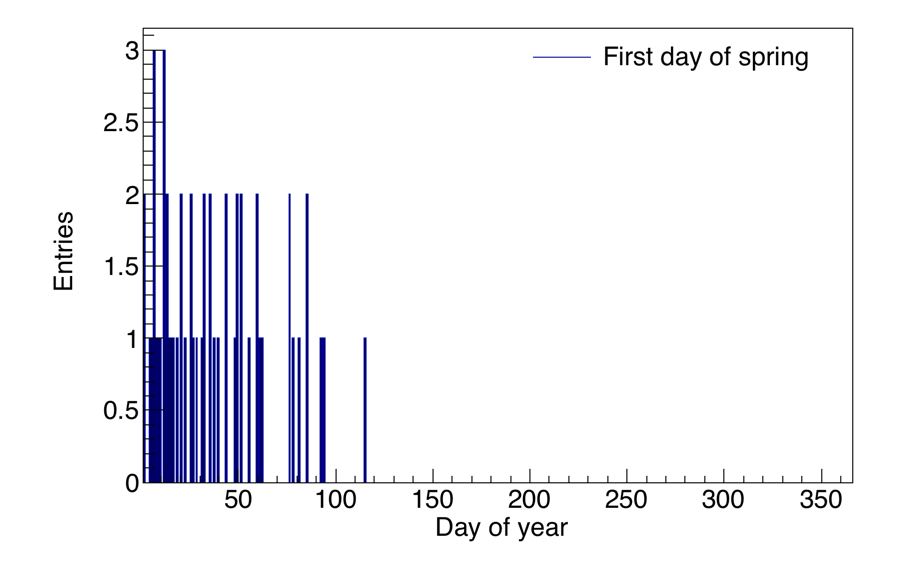
\includegraphics[width=0.5\textwidth]{springHistogram.png}}\\
\caption{The first day on which spring starts for each year in Lund is shown in (a).  While (b) shows the number of times spring starts on a certain day in the year.}
\label{fig:spring}
\end{figure}

\begin{figure}[ht!]
\centering
\subfloat[Bar graph]{\label{fig:summer_bar}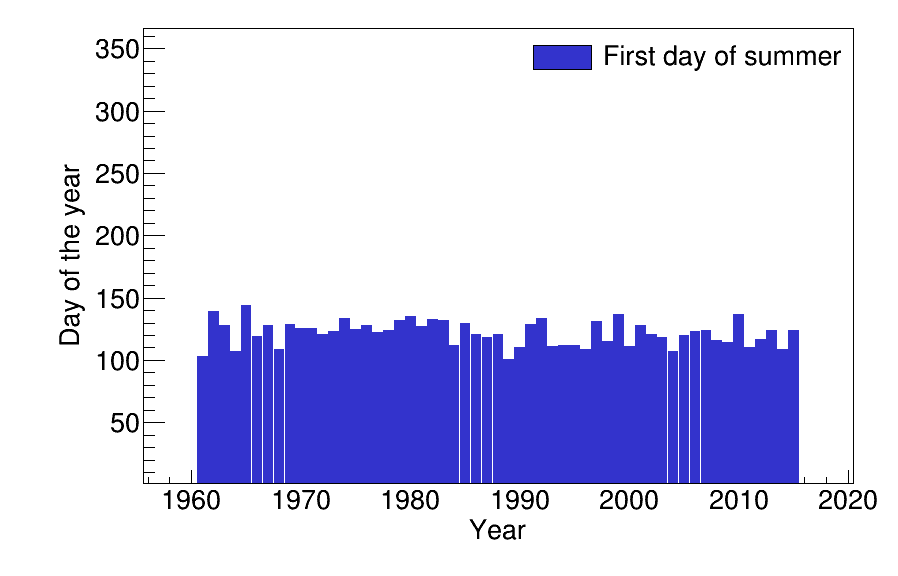
\includegraphics[width=0.5\textwidth]{summerStart.png}} 
\subfloat[Histogram]{\label{fig:summer_hist}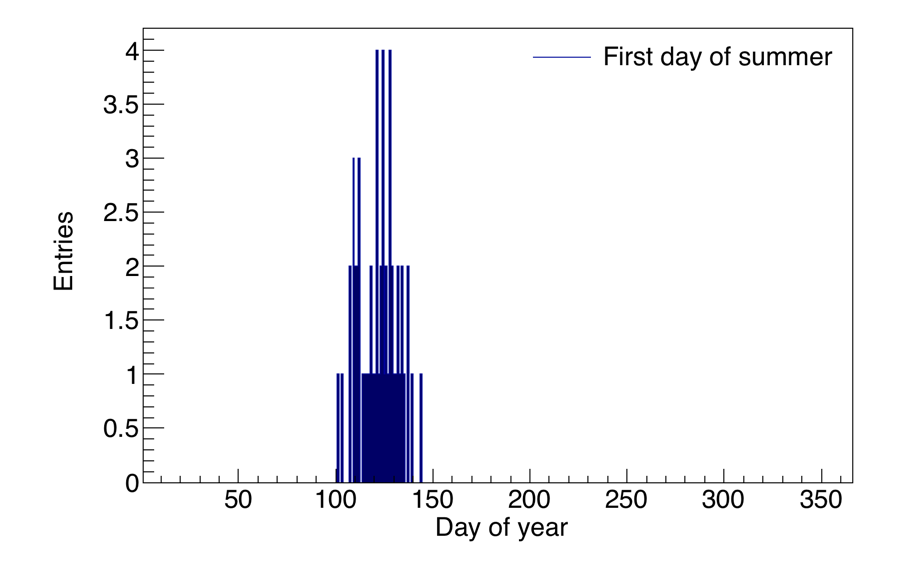
\includegraphics[width=0.5\textwidth]{summerHistogram.png}}\\
\caption{The first day on which summer starts for each year in Lund is shown in (a).  While (b) shows the number of times summer starts on a certain day in the year.}
\label{fig:summer}
\end{figure}

\begin{figure}[ht!]
\centering
\subfloat[Bar graph]{\label{fig:fall_bar}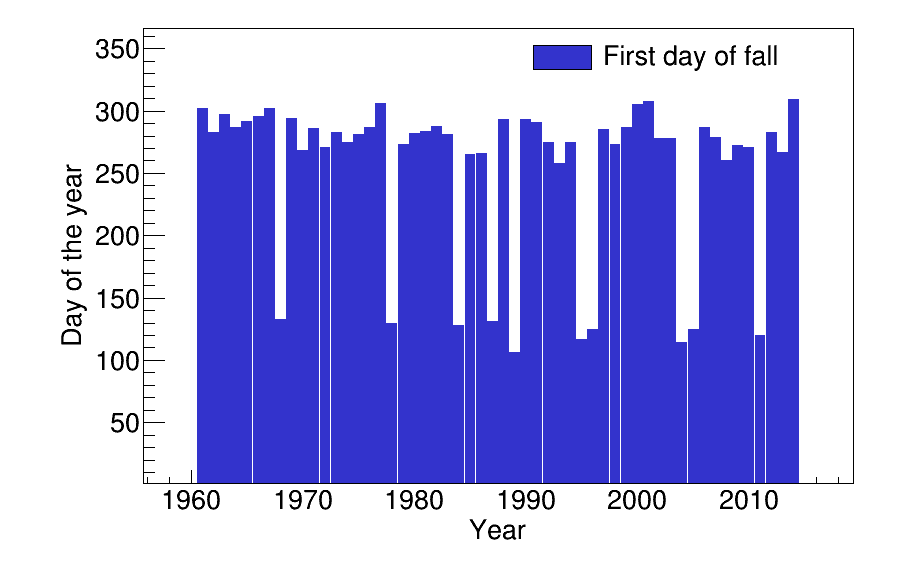
\includegraphics[width=0.5\textwidth]{fallStart.png}} 
\subfloat[Histogram]{\label{fig:fall_hist}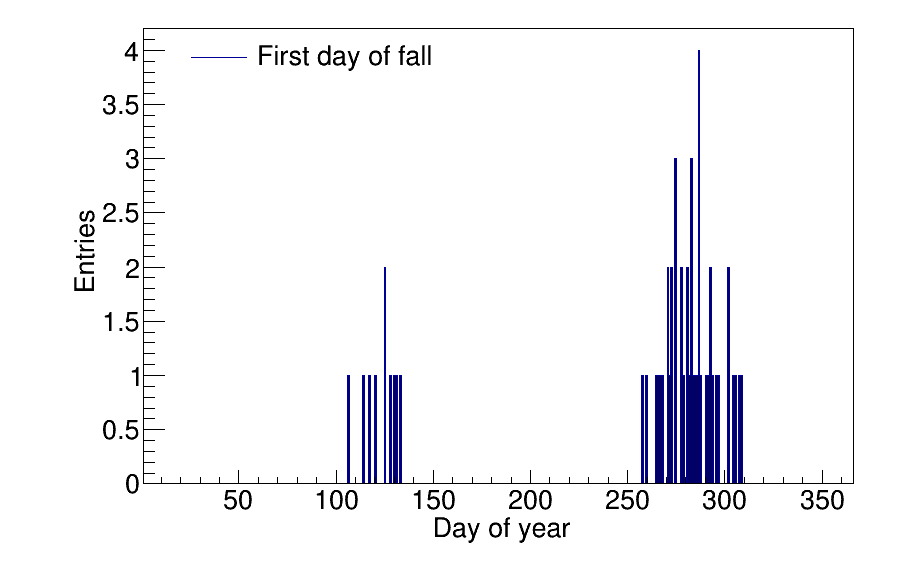
\includegraphics[width=0.5\textwidth]{fallHistogram.png}}\\
\caption{The first day on which fall starts for each year in Lund is shown in (a).  While (b) shows the number of times summer starts on a certain day in the year.}
\label{fig:fall}
\end{figure}

\begin{figure}[ht!]
\centering
\subfloat[Bar graph]{\label{fig:winter_bar}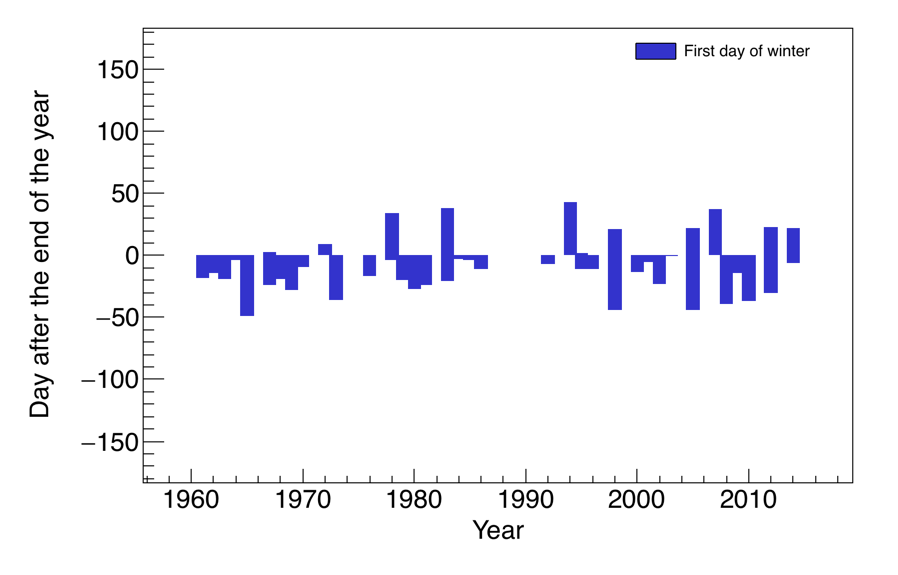
\includegraphics[width=0.5\textwidth]{winterStart.png}} 
\subfloat[Histogram]{\label{fig:winter_hist}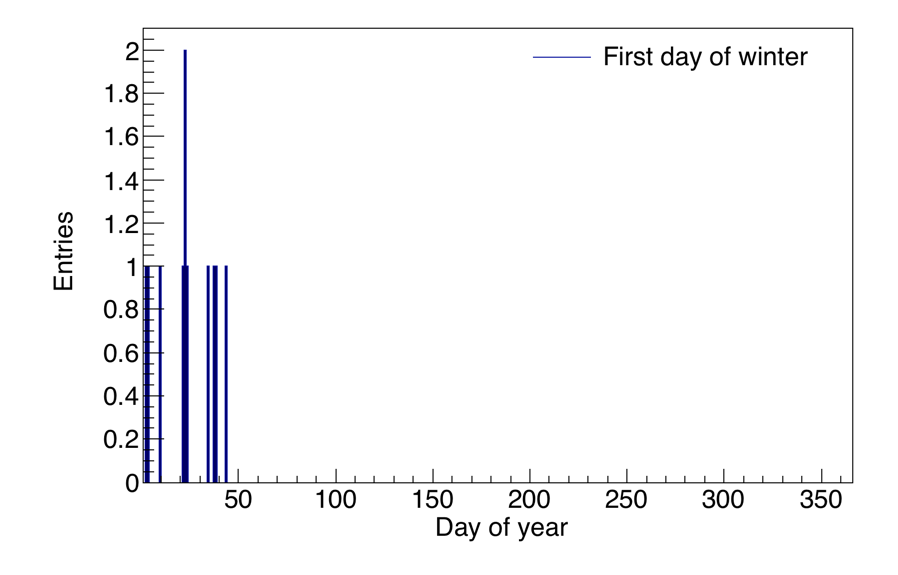
\includegraphics[width=0.5\textwidth]{winterHistogram.png}}\\
\caption{The first day on which winter starts for each year in Lund is shown in (a). The day is given relative to the start of a new year, all negative numbers are before the $1^{\text{st}}$ of January and all the positive numbers are on or after the $1^\text{st}$ of January.  The number of times spring starts on a certain day in the year in given in (b).}
\label{fig:winter}
\end{figure}

\end{document}















